
\documentclass[12pt]{report}
\usepackage[a4paper]{geometry}
\usepackage[myheadings]{fullpage}
\usepackage{fancyhdr}
\usepackage{lastpage}
\usepackage{graphicx, wrapfig, subcaption, setspace, booktabs}
\usepackage[T1]{fontenc}
\usepackage[font=small, labelfont=bf]{caption}
\usepackage{fourier}
\usepackage[protrusion=true, expansion=true]{microtype}
\usepackage[english]{babel}
\usepackage{sectsty}
\usepackage{url, lipsum}
\usepackage{tgbonum}
\usepackage{hyperref}
\usepackage{xcolor}

\newcommand{\HRule}[1]{\rule{\linewidth}{#1}}
\onehalfspacing
\setcounter{tocdepth}{5}
\setcounter{secnumdepth}{5}


\begin{document}
{\fontfamily{cmr}\selectfont
\title{ \normalsize \textsc{}
		\\ [2.0cm]
		\HRule{0.5pt} \\
		\LARGE \textbf{\uppercase{Project 2}
		\HRule{2pt} \\ [0.5cm]
		\large CS691 \\
		\normalsize Due Date : October 19, 2019 \\
		\vspace*{5\baselineskip}
		}
		}


\author{
		Sharif Kamran \\
		Adam Lychuk \\
}

\maketitle
\tableofcontents
\newpage

\sectionfont{\scshape}

\section{Task 1}
\subsection{KNN\textunderscore test(X\textunderscore train,Y\textunderscore train,X\textunderscore test,Y\textunderscore test,K)}
The function takes the training and test samples along with the labels and the K as input to build a k-nearest neighbor. For each of the test samples we iterate and find the k nearest sample with respect to that test case. As a result, we calculate the euclidean distance using \textbf{Calculate\textunderscore distance} function from the each of the training cases from that particular test case and append it into an array. After that we sort the array with \textbf{sorted\textunderscore neighbor} function and keep a tracker for the indexes. This will help us to track the labels (signs) of each of the training case later on and find the majority sign (positive or negative) for that particular test case. For finding the sign of the majority case we use the \textbf{sign\textunderscore pred} function and append the prediction to an array. After that, we call the \textbf{Accuracy} function send the prediction values and Y\textunderscore test as input to get the overall accuracy.

\subsection{Results: Predictions for K=1, K=3 and K=5}
\begin{table}[h]
\centering
\begin{tabular}{|c|c|c|c|}
\hline
\textbf{True label} & \textbf{K=1} & \textbf{K=3} & \textbf{K=5} \\ \hline
1          & -1           & 1            & 1            \\ \hline
-1         & 1            & 1            & -1           \\ \hline
1          & 1            & 1            & -1           \\ \hline
-1         & -1           & -1           & 1            \\ \hline
1          & -1           & -1           & -1           \\ \hline
-1         & 1            & -1           & -1           \\ \hline
1          & 1            & 1            & 1            \\ \hline
-1         & 1            & 1            & 1            \\ \hline
1          & -1           & -1           & 1            \\ \hline
-1         & 1            & 1            & -1           \\ \hline
Accuracy   & 30\%         & 40\%         & 60\%         \\ \hline
\end{tabular}
\end{table}


\subsection{choose\textunderscore K(X\textunderscore train,Y\textunderscore train,X\textunderscore val,Y\textunderscore val)}
The function takes the training and validation samples as input and tries to find the best K for the give validation samples (test). For this it iterates from $K=1$ to $K=number of training samples$ and then calls the \textbf{KNN\textunderscore test} function as finds the accuracy for each of the sample. It also keeps the best accuracy for the given K so that it can return it as the best K for the test samples. 

\subsection{Best K}
The best K for given test sample is 9. With accuracy of 70\% this is the best performing K among all the values from 1 to 13.


\section{Task 2}
\subsection{K\textunderscore Means(X,K)}
This function performs the K-Means algorithm. The function takes the samples, which can be any set of n-dimensional feature vectors, and assigns each to a random class. The number of classes is decided by the number of centers which is decided by input K. After this initialization the algorithm runs for an arbitrary 100 iterations in the hopes of convergence. Each iteration the function finds the distance between each cluster center and each sample point. It then assigns points to the initialized classes based on the center they're closest too. At the end of this process we check to see if any points have been reassigned to classes. If no points have been reassigned, k-means converged. Otherwise we compute new centers, by taking the mean of points in each class, and assigning that mean as the new center.
\subsection{K\textunderscore Means\textunderscore better(X,K)}
This function calls K\textunderscore Means(X,K) until center values are found that are generally the same. Once it identifies those centers it returns them.

\section{Task 3}
\subsection{perceptron\textunderscore train(X,Y)}
The function takes training sample sand labels as input and then iterates over them and optimizes the weights and the bias. First \textbf{weight\textunderscore initialize} function is called where random weights are initialize with values of $[-1,1]$ with four decimal places. After that we iterate for 10 epochs to take one sample each time and do Dot product operation between the weight and the samples. After that we calculate if the activation is bigger than zero or not. If not then we update both the weights and the bias. The activation is calculated using the \textbf{activation} function and the weights are updated by calling \textbf{update\textunderscore weights} function. We return all the weight value along with the bias at the end of the function. 


\subsection{perceptron\textunderscore test(X\textunderscore test, Y\textunderscore test, w, b)} 
The function uses testing samples and labels along with weights and biases as input and finds the overall accuracy. First it iterates through the test samples and using the \textbf{activation} function finds the prediction and appends it into an array. Then it matches the prediction to the true label and finds how many of them are correct. Lastly, it finds the the overall accuracy in terms of percentage and returns it.
}

\begin{figure}[h]
    \centering
    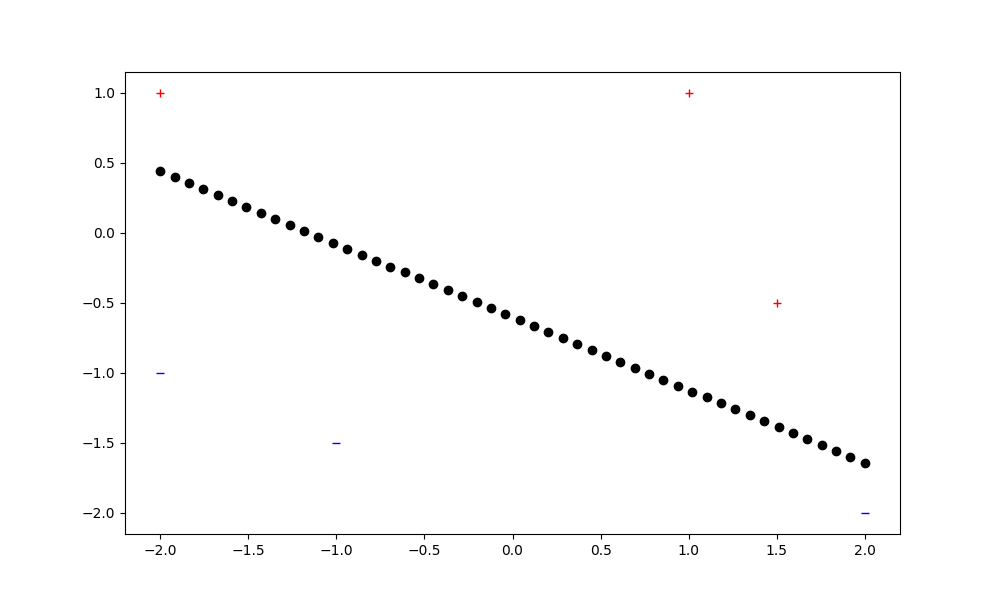
\includegraphics[width=1.1\textwidth]{plot.png}
    \caption{Decision Boundary}
    \label{Decision Boundary}
\end{figure}{}
\end{document}

